\renewcommand*\chappic{img/diff-crypt.pdf}
\renewcommand*\chapquote{Just because it's automatic doesn't mean it works.}
\renewcommand*\chapquotesrc{Daniel J. Bernstein}
\chapter{Differential cryptanalysis}
\label{ch:dc}
%
\section{MD4}
\label{sec:dc-md4}
%
MD4 is a cryptographic hash function originally described in RFC~1186~\cite{rfc1186},
updated in RFC~1320~\cite{rfc1320} and declared obsolete by RFC~6150~\cite{rfc6150}. It was
invented by Ronald Rivest in 1990 with properties given in Table~\ref{tab:md4}.
Since 1995~\cite{Dobbertin1998} successful attacks have been found to break collisions,
preimage and second-preimage resistance in MD4; including but not limited to~\cite{md4-2007} and
\cite{cryptoeprint:2005:151}. A Python~3 implementation derived from a previous Python version
is available at github~\cite{md4-py3k}.

\begin{table}[h]
  \begin{center}
    \begin{tabular}{lcl}
      block size           & 512 bits       & namely variable \texttt{block} in RFC~1320~\cite{rfc1320} \\
      digest size          & 128 bits       & as per section~3.5 in RFC~1320~\cite{rfc1320} \\
      internal state size  & 128 bits       & namely variables $A$, $B$, $C$ and $D$ \\
      word size            & 32 bits        & as per section~2 in RFC~1320~\cite{rfc1320} \\
    \end{tabular}
    \caption{MD4 hash algorithm properties}
    \label{tab:md4}
  \end{center}
\end{table}

In the following a quick overview over MD4's design is given.

First of all, padding is applied. A single bit 1 is appended to the
input. As long as the input does not reach a length congruent 448 modulo 512,
bit 0 is appended.
Followingly, length appending takes place. Represent the length of the input
(without the modifications of the previous step) in binary and take its first
64 bits. Append those 64 bits to the input.

The message is split into 512-bit blocks (i.e. 16 32-bit words).
Four state variables $A$, $B$, $C$ and $D$ are initialized with hexadecimal values:
\[
  \mathbf{[A]}\; \mathtt{01234567} \quad
  \mathbf{[B]}\; \mathtt{89abcdef} \quad
  \mathbf{[C]}\; \mathtt{fedcba98} \quad
  \mathbf{[D]}\; \mathtt{76543210}
\]
To process one block, three auxiliary boolean functions are defined:
\begin{align}
  \IF(X,Y,Z) &= (X \land Y) \lor (\neg X \land Z) \\
  \MAJ(X,Y,Z) &= (X \land Y) \lor (X \land Z) \lor (Y \land Z) \\
  \XOR(X,Y,Z) &= X \oplus Y \oplus Z
\end{align}

\begin{defi}
  The boolean $\IF$ function behaves the following way:
  If the first argument is true, the second argument is returned.
  If the first argument is false, the third argument is returned.

  The boolean $\MAJ$ function returns true if the number
  of boolean values true in arguments is at least $2$.
  The boolean $\XOR$ function returns true if the number
  of boolean values true in arguments is odd.
\end{defi}

\begin{figure}[t]
  \begin{center}
    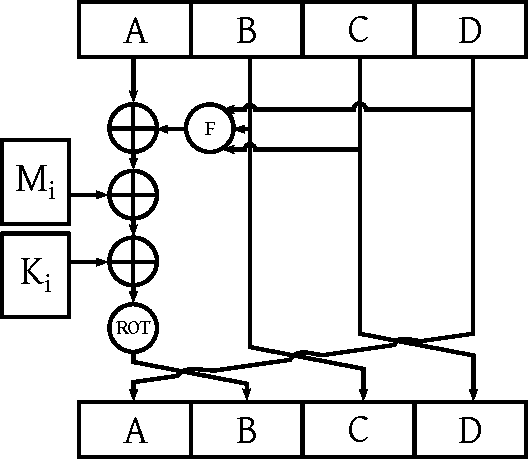
\includegraphics{img/md4.pdf}
    \caption{MD4 round function}
    \label{fig:md4-round-function}
  \end{center}
\end{figure}

\section{SHA-256}
\label{sec:dc-sha-256}

% Merkle–Damgård construction

\begin{figure}[t]
  \begin{center}
    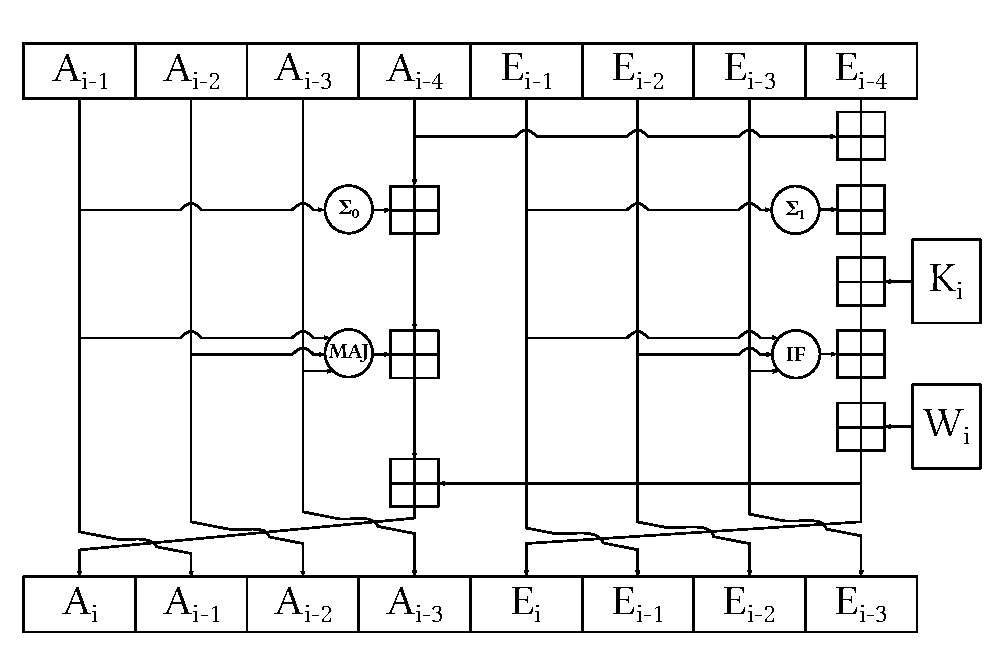
\includegraphics{img/sha256.pdf}
    \caption{SHA-256 round function}
    \label{fig:sha256-round-function}
  \end{center}
\end{figure}

\section{Differential notation}
\label{sec:dc-notation}
%
\cite{char-2006}


\section{Addition example}
\section{Differential path}
